\section{genericTPGVcs.h File Reference}
\label{genericTPGVcs_8h}\index{genericTPGVcs.h@{genericTPGVcs.h}}
{\tt \#include \char`\"{}genericInterface.h\char`\"{}}\par
{\tt \#include \char`\"{}genericEvents.h\char`\"{}}\par
{\tt \#include \char`\"{}../../../util/genericData.h\char`\"{}}\par
{\tt \#include \char`\"{}../interfaces/processor.h\char`\"{}}\par
{\tt \#include \char`\"{}../../data\_\-types/impl/highLevelPacket.h\char`\"{}}\par
{\tt \#include \char`\"{}../../../memctrl/request.h\char`\"{}}\par
{\tt \#include \char`\"{}../../../memctrl/mshr.h\char`\"{}}\par
{\tt \#include \char`\"{}../../../util/mc\_\-constants.h\char`\"{}}\par
{\tt \#include $<$math.h$>$}\par
{\tt \#include $<$fstream$>$}\par
{\tt \#include $<$deque$>$}\par


Include dependency graph for genericTPGVcs.h:\nopagebreak
\begin{figure}[H]
\begin{center}
\leavevmode
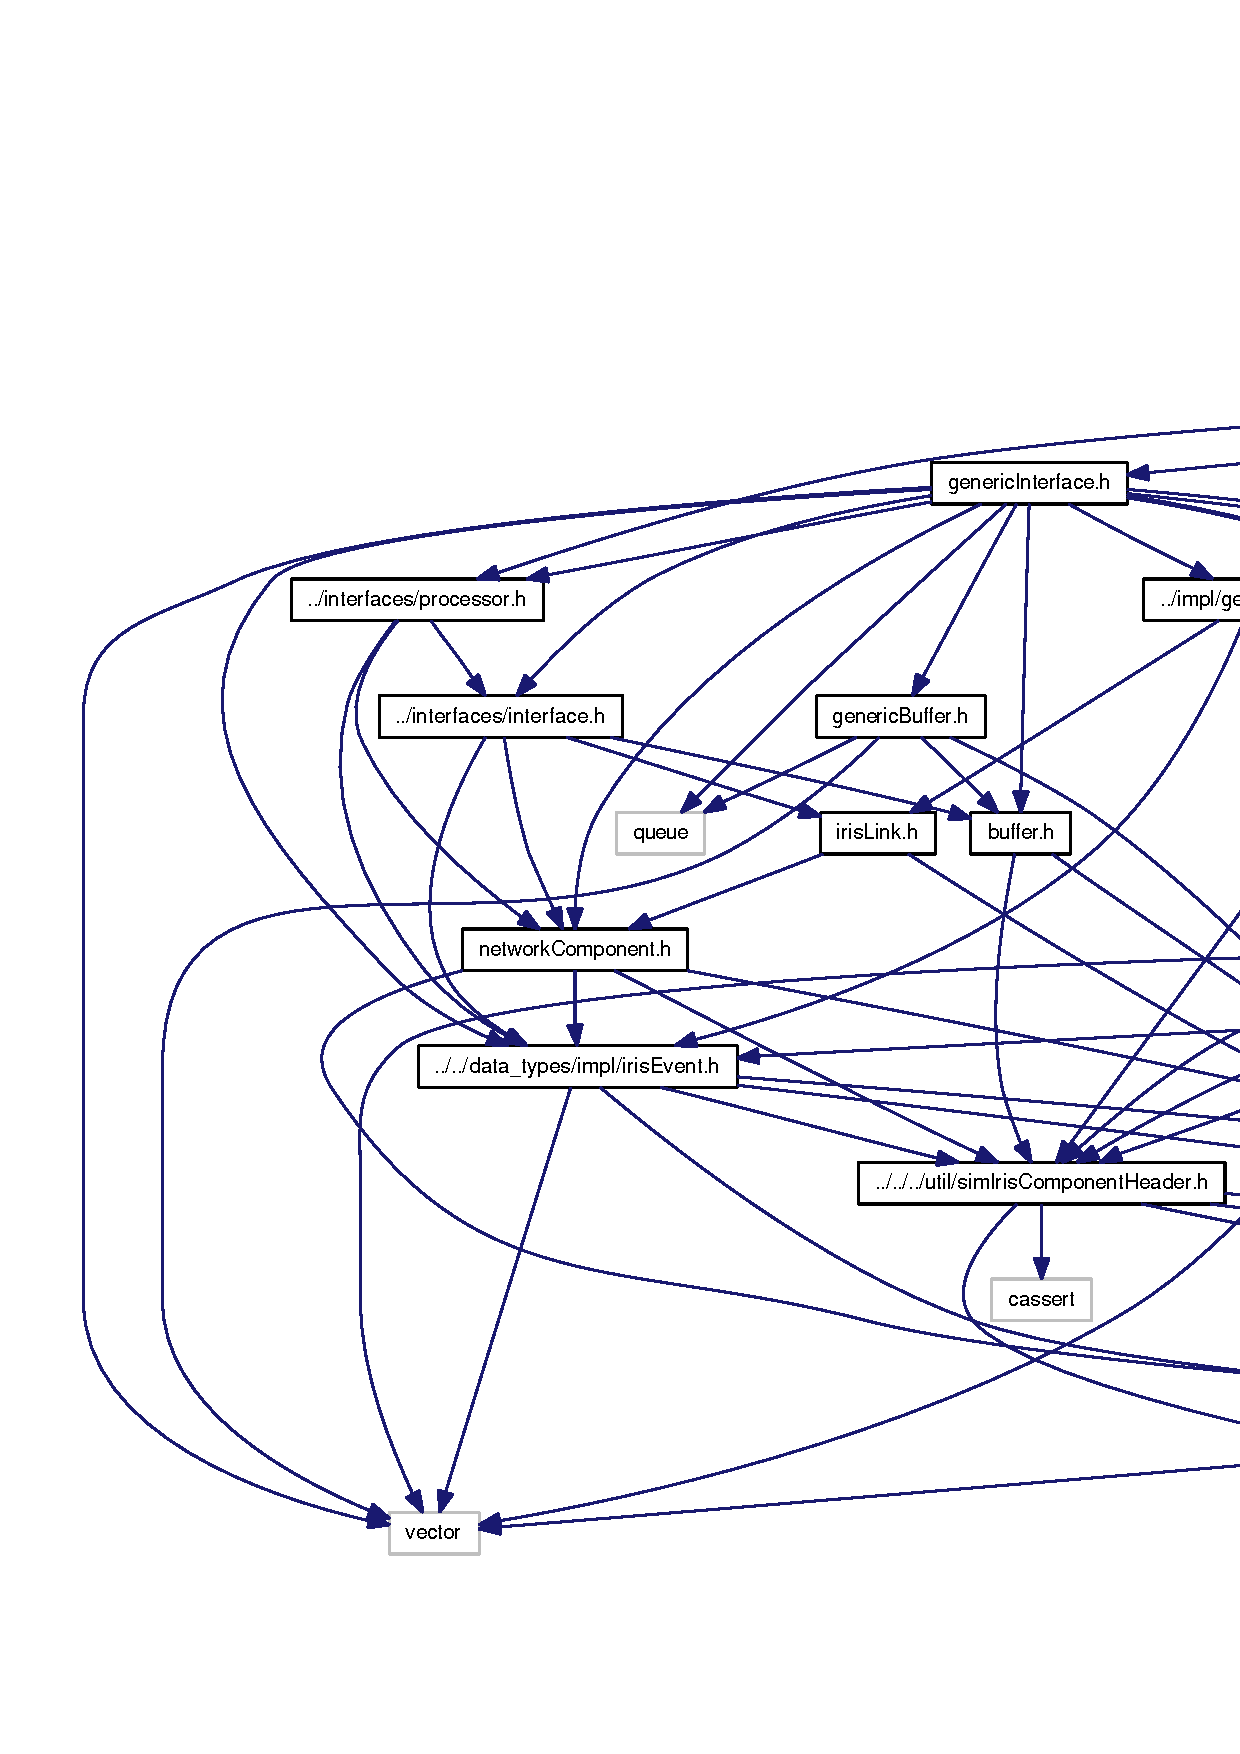
\includegraphics[width=420pt]{genericTPGVcs_8h__incl}
\end{center}
\end{figure}


This graph shows which files directly or indirectly include this file:\nopagebreak
\begin{figure}[H]
\begin{center}
\leavevmode
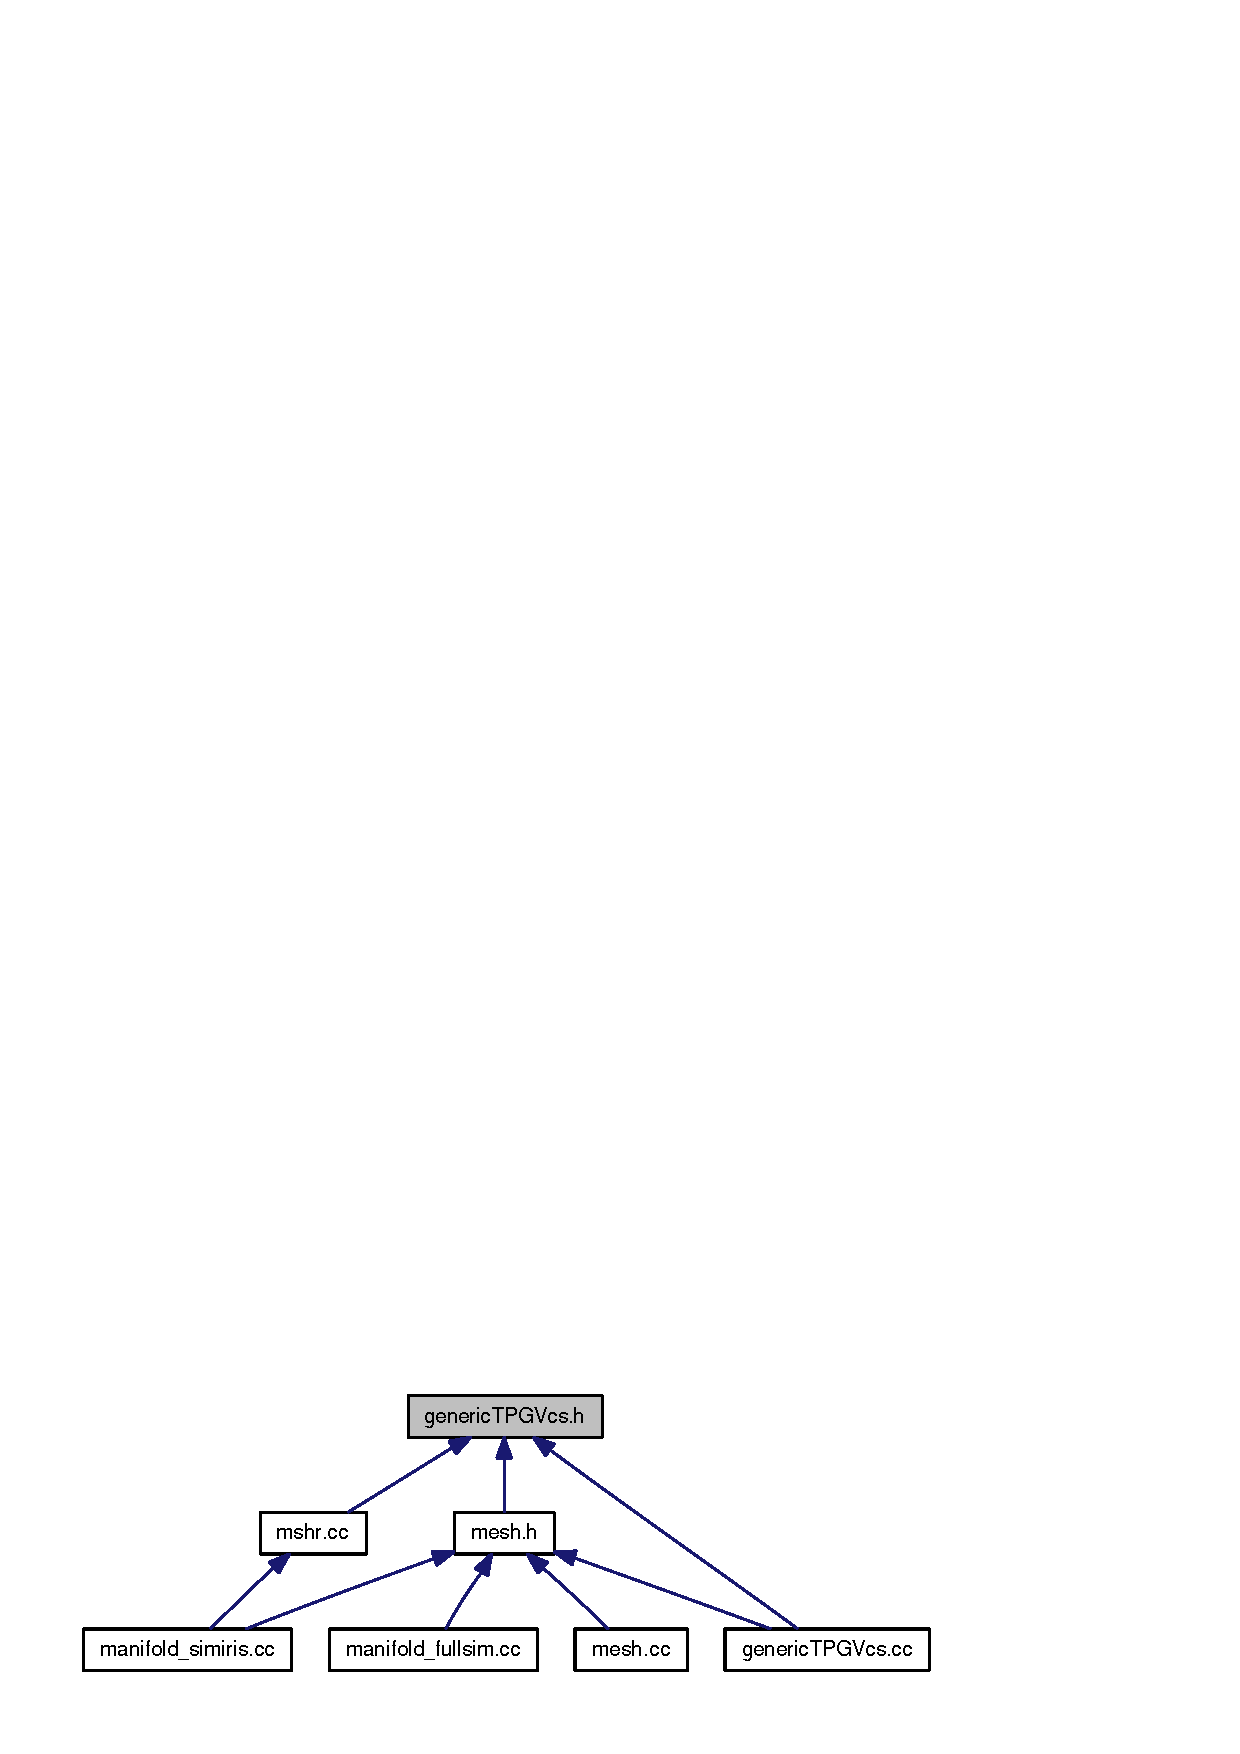
\includegraphics[width=225pt]{genericTPGVcs_8h__dep__incl}
\end{center}
\end{figure}
\subsection*{Classes}
\begin{CompactItemize}
\item 
class {\bf GenericTPGVcs}
\end{CompactItemize}
\subsection*{Defines}
\begin{CompactItemize}
\item 
\#define {\bf DEFAULT\_\-RAN\_\-MAX\_\-TIME}~100
\item 
\#define {\bf MAX\_\-ADDRESS}~3
\end{CompactItemize}
\subsection*{Variables}
\begin{CompactItemize}
\item 
{\bf uint} {\bf no\_\-nodes}
\item 
{\bf uint} {\bf no\_\-mcs}
\end{CompactItemize}


\subsection{Define Documentation}
\index{genericTPGVcs.h@{genericTPGVcs.h}!DEFAULT\_\-RAN\_\-MAX\_\-TIME@{DEFAULT\_\-RAN\_\-MAX\_\-TIME}}
\index{DEFAULT\_\-RAN\_\-MAX\_\-TIME@{DEFAULT\_\-RAN\_\-MAX\_\-TIME}!genericTPGVcs.h@{genericTPGVcs.h}}
\subsubsection[{DEFAULT\_\-RAN\_\-MAX\_\-TIME}]{\setlength{\rightskip}{0pt plus 5cm}\#define DEFAULT\_\-RAN\_\-MAX\_\-TIME~100}\label{genericTPGVcs_8h_95a6218d50e244f6e58b6cca098c1d65}




Definition at line 17 of file genericTPGVcs.h.\index{genericTPGVcs.h@{genericTPGVcs.h}!MAX\_\-ADDRESS@{MAX\_\-ADDRESS}}
\index{MAX\_\-ADDRESS@{MAX\_\-ADDRESS}!genericTPGVcs.h@{genericTPGVcs.h}}
\subsubsection[{MAX\_\-ADDRESS}]{\setlength{\rightskip}{0pt plus 5cm}\#define MAX\_\-ADDRESS~3}\label{genericTPGVcs_8h_aba07841c3e227bc8bdd8ccdad149349}




Definition at line 18 of file genericTPGVcs.h.

\subsection{Variable Documentation}
\index{genericTPGVcs.h@{genericTPGVcs.h}!no\_\-mcs@{no\_\-mcs}}
\index{no\_\-mcs@{no\_\-mcs}!genericTPGVcs.h@{genericTPGVcs.h}}
\subsubsection[{no\_\-mcs}]{\setlength{\rightskip}{0pt plus 5cm}{\bf uint} {\bf no\_\-mcs}}\label{genericTPGVcs_8h_56d27d790e05179f3787fce80d802d04}




Definition at line 31 of file config\_\-params.h.\index{genericTPGVcs.h@{genericTPGVcs.h}!no\_\-nodes@{no\_\-nodes}}
\index{no\_\-nodes@{no\_\-nodes}!genericTPGVcs.h@{genericTPGVcs.h}}
\subsubsection[{no\_\-nodes}]{\setlength{\rightskip}{0pt plus 5cm}{\bf uint} {\bf no\_\-nodes}}\label{genericTPGVcs_8h_b78c10782810279fb9680eafef33b77d}




Definition at line 30 of file config\_\-params.h.